\documentclass{article}
\usepackage[T1]{fontenc}
\usepackage [ english ]{ babel }
\usepackage[utf8]{inputenc}
\usepackage{mathtools}
\usepackage{graphicx}
\usepackage{setspace}
\graphicspath{ {images/} }

\title{Parallel Computing report}
\author{Andrea Costalonga}
\date{20/08/2021}

\begin{document}
\maketitle
\textbf{\LARGE Parallelizing Quicksort}
\section{Introduction}
Among the algorithms used for sorting, quicksort is one of the main actors. It's performances 
are known to be comparable to the mergesort ones ($T(N) = O(N*log(N))$ mainly, $O(N^2)$ in the worst case) 
and, as we will see, also its parallel performances are not far from $T(N,P) = O(\frac{N}{P}*log(\frac{N}{P}))$.
\\The algorithm can be described with the following recursive formulation:
\begin{enumerate}
    \item If the istance has at most one element, return;(base case)
    \item Otherwise pick a element among the ones in the instance, that will be the PIVOT;
    \item Separate the elements greater than the PIVOT (right subgroup) from the others(left subgroup);
    \item Apply recursively the algorithm to the left and right subgroups;
\end{enumerate}
There are various methods to pick the pivot: chosen at random, picked from the back or 
picking the median of a subgroup,etc\dots; in this implementation I've gone for the second option.
The usual implementation of the quicksort works \textit{In Loco}, switching the position between the elements
of the input array. In my version I've used stacks implemented via linked lists: it's a questionable choice
but I really liked the challenge and the urge of doing something different from my colleagues.

\section{Parallel-ify}
I tried to parallelize the algorithm in the following way:
\begin{enumerate}
    \item Partitioning the input in P partitions;(with P := \# of processors)
    \item Applying the sequential algorithm to those partitions;
    \item Merging the partitions toghether;
\end{enumerate}

Surprisingly this procedure worked flawlessly so I've gone for it. Pragmatically speaking the partitioning of 
the instance has been done through the method $MPI\_Scatter()$ and the merging steps using the basic
methods $MPI\_Send()$ and $MPI\_Recv()$.

\subsection*{Analysis}
For simplicity from now on we will consider N(:= instance size) a multiple of P 
and P a power of 2.\\
We can start analysing the performances of the sequential algorithm running on the 
$n = \frac{N}{P}$ sized partitions. We can easilly state that in the average case
$T\textsubscript{sort}(n) = O(n*log(n))$ since we are just applying the sequential algorithm for a 
smaller instance.\\ 
The parallel merger, instead, works merging in parallel couples of partitions going from P partitions to 1. 
With a good approximation we can assume that a good serial merging algorithm can merge two $n/2$ arrays in time 
$T\textsubscript{merge}(n) = n$.  
Given the hypothesys above we can write without loss of generality the following equation:
\begin{equation}
T\textsubscript{merge}(N,P) =\sum_{i=0}^{log_2(P)-1}(T\textsubscript{merge}(\frac{N}{2^i})) \le 2N = O(N) 
\end{equation}
Knowing that $T(N,P) = T\textsubscript{merge}(N,P) + T\textsubscript{sort}(\frac{N}{P})$ we can naturally derive
\begin{equation}
T(N,P) = O(\frac{N}{P}*log(\frac{N}{P})) + O(N) = O(\frac{N}{P}*log(\frac{N}{P}))
\end{equation}
since $\lim_{N \to \inf}\frac{N}{\frac{N}{P}*log(\frac{N}{P}))} = 0$ for any fixed P > 0, and if $f(n) \in o(n)$ then $f(n) \in O(n)$.\\
Things work similarly for the worst case scenario, since we can just assume $T\textsubscript{sort}(n) = O(n^2)$, obtaining 
$T(N,P) = O((\frac{N}{P})^2)$.
\pagebreak
\section{Experimental Analysis}
Below there are some results obtained running the algorithms on HPC Capri, every 
job used the same amount of RAM, 12gb.\\
\subsection*{Optimizations}
First of all I've started checking if I could tweak the algorithm in some way to obtain better
performances. I've tryed to run the algorithm without compiler optiminzations and then using 
O1, O2, O3.\\
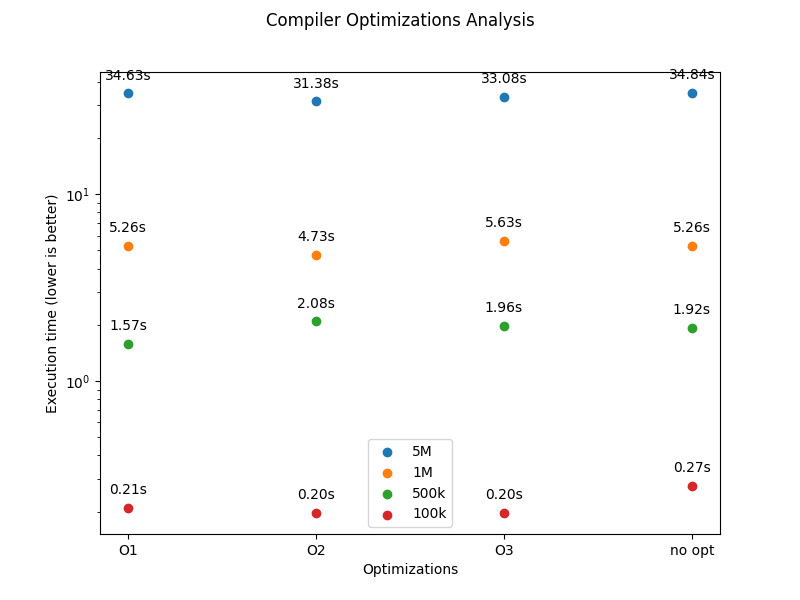
\includegraphics[scale=.6]{opt_boxplot.png}
As we can see there's not much difference between the 4 different cases, still in the overall results
O2 behaved quite well, so I've decided to use it for the following tests. In the plot I've showed the results for
the sequential algorithm, the parallel algorithm behaved very similarly so I've preferred to omit the analysis
for the MPI implementation.
\subsection*{Execution Times}
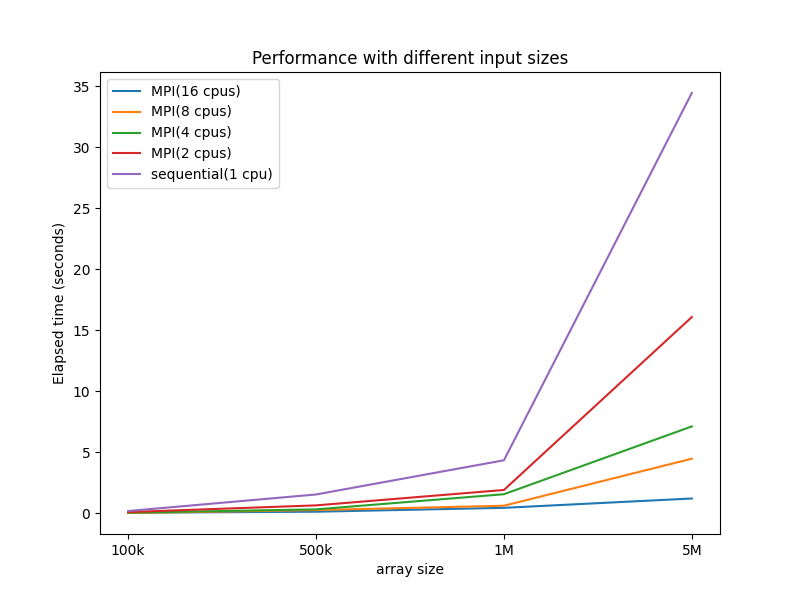
\includegraphics[scale=.6]{inputsChart.png}
In the experiments I've used 4 different text-files containing a increasing amount of elements: 
100k, 500k, 1M, 5M. Every element in those files is a floating point number (float). The graph 
above shows the running time of the quicksort algorithm: what we can clearly see is the great 
difference between the sequential algorithm and the optimized version running with 2, 4, 8 and 16 
cores; the used optimization for both the standard and the parallelized algorithm is '-O2' as 
mentioned above. Every step, going from 2 to 16 cores, brought better results in terms of running 
time, with a maximum speedup rateo of 28 (16 cores with the 5M file, more info in the fourth chart). 
A better illustration of the results using a logarithmic scale on the time axis can be found below.  

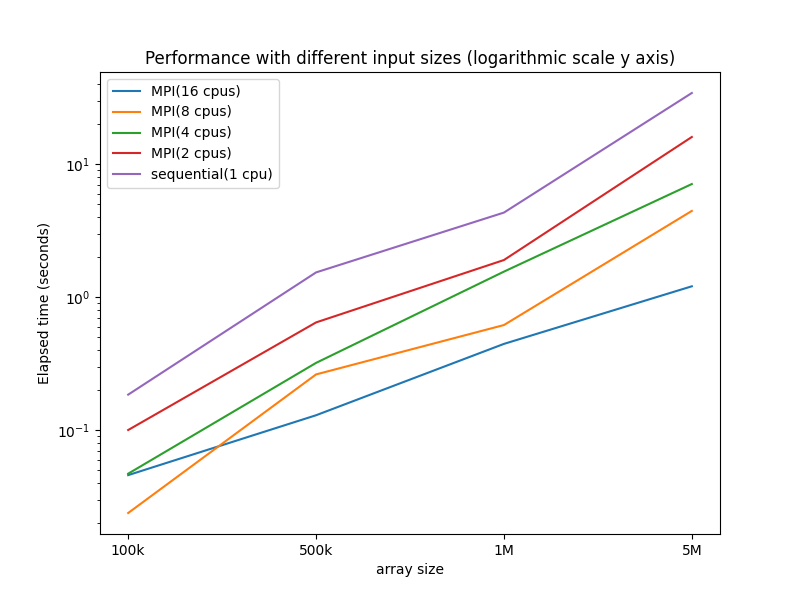
\includegraphics[scale=.6]{inputsChartLog.png}
Here in the last image I've plotted some results about speedup:\\
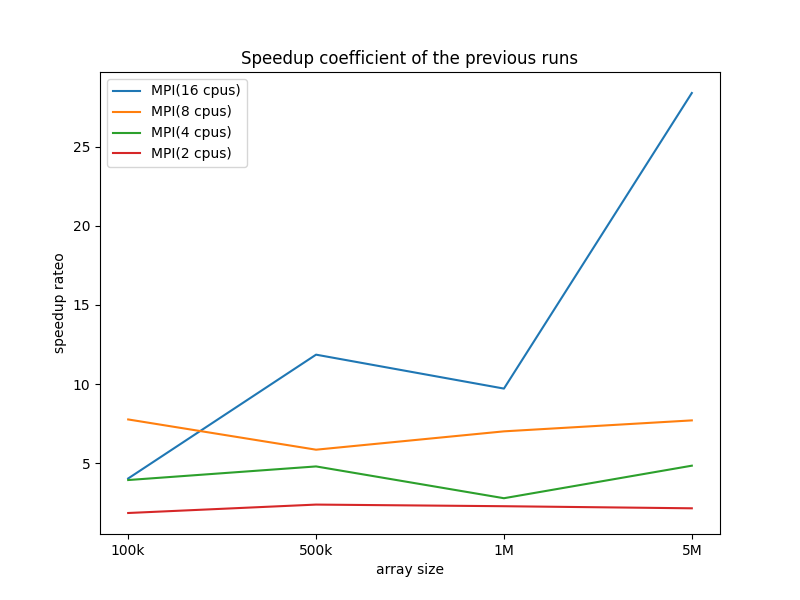
\includegraphics[scale=.6]{speedup.png}
With this last plot I wanted to show the different speedups obtained in the test runs, and it's easy 
to see that having a higher number of processors in this case makes the algorithm run faster, and
it's a good occasion to point out that this algorithm, Quicksort, behaves very nicely when trying 
to parallelize it. The results follow quite nicely the predicted speedup.

\section{Final Considerations}
It has been a good challenge trying to implement a performing version of quicksort; the entire 
repository with the final version of the algorithm can be found here: https://github.com/Starkiller13/ParallelQuicksortMPI.
In the repository you will find a Readme.md with everything needed to compile and run the algorithm.

\section{Bibliography}
\begin{enumerate}
    \item Ideas for the parallelization process and recap of quicksort:\\
    https://cse.buffalo.edu/faculty/miller/Courses/CSE633/Sri-Abinaya-Gunasekaran-Spring-2019.pdf
    \item Linked list Stack implementation:\\
    https://www.educative.io/edpresso/how-to-implement-a-stack-in-c-using-a-linked-list
    \item Python plot library used for the plots:\\
    https://matplotlib.org/
    \item C documentation:\\
    https://devdocs.io/c/
\end{enumerate}
\end{document}
